\documentclass[12pt]{article}
\usepackage{amsfonts}
\usepackage{fancyhdr}
\usepackage[a4paper, top=2.5cm, bottom=2.5cm, left=2.2cm, right=2.2cm]{geometry}
\usepackage{times}
\usepackage{amsmath}
\usepackage{changepage}
\usepackage{amssymb}
\usepackage{graphicx}%
\setcounter{MaxMatrixCols}{30}
\newtheorem{theorem}{Theorem}
\newtheorem{acknowledgement}[theorem]{Acknowledgement}
\newtheorem{algorithm}[theorem]{Algorithm}
\newtheorem{axiom}{Axiom}
\newtheorem{case}[theorem]{Case}
\newtheorem{claim}[theorem]{Claim}
\newtheorem{conclusion}[theorem]{Conclusion}
\newtheorem{condition}[theorem]{Condition}
\newtheorem{conjecture}[theorem]{Conjecture}
\newtheorem{corollary}[theorem]{Corollary}
\newtheorem{criterion}[theorem]{Criterion}
\newtheorem{definition}[theorem]{Definition}
\newtheorem{example}[theorem]{Example}
\newtheorem{exercise}[theorem]{Exercise}
\newtheorem{lemma}[theorem]{Lemma}
\newtheorem{notation}[theorem]{Notation}
\newtheorem{problem}[theorem]{Problem}
\newtheorem{proposition}[theorem]{Proposition}
\newtheorem{remark}[theorem]{Remark}
\newtheorem{solution}[theorem]{Solution}
\newtheorem{summary}[theorem]{Summary}
\usepackage{enumitem}
\usepackage[utf8]{inputenc}
\newenvironment{proof}[1][Proof]{\textbf{#1.} }{\ \rule{0.5em}{0.5em}}
\usepackage{tikz}
\usetikzlibrary{fit,arrows,calc,positioning}
\usepackage{graphicx}
\usepackage{wrapfig}
\usepackage{float}
\usepackage{datetime}
\newdateformat{specialdate}{\twodigit{\THEDAY}.\twodigit{\THEMONTH}.\THEYEAR}
\usepackage{amssymb}
\usepackage{ifsym}
\usepackage{mathtools}
\usepackage{listings}
\usepackage{lipsum}  

\newcommand{\blue}[1]{\color{blue}#1\color{black}}
\newcommand{\red}[1]{\color{red}#1\color{black}}
\newcommand{\green}[1]{\color{green}#1\color{black}}
\newcommand{\N}{\mathbb{N}}
\newcommand{\Q}{\mathbb{Q}}
\newcommand{\R}{\mathbb{R}}
\newcommand{\C}{\mathbb{C}}
\newcommand{\Z}{\mathbb{Z}}
\renewcommand\labelenumii{\theenumi.\arabic{enumii}.}
\newcommand{\code}[1]{\texttt{#1}}

\begin{document}
	
	\title{7. Exercise}
	\author{Timo Bergerbusch 344408 \\ Thomas Näveke 311392 \\ Shu Xing 381176}
	\date{\specialdate\today}
	\maketitle
	
	\section*{Exercise 7.1(Schedules, Serializability, and Locking)}
	\subsection*{7.1.1}
		The schedule is not conflict serializable, because its corresponding conflict graph is cyclic.\\
		With the $conflict(s_0)$=$\lbrace(w_0(A), r_1(A)),(r_1(B), w_0(B))\rbrace$:
		
		\begin{figure}[H]
		\centering
		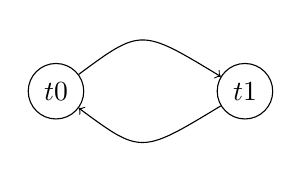
\begin{tikzpicture}[node distance = 3cm,scale=.8, every node/.style={circle,anchor=west}]
			\node[draw] (v1) at (0,0) {$t0$};
			\node[draw] (v2) at (3,0) {$t1$};
			\draw[->] (v1) .. controls (1.8, 1)  ..  (v2) ;		
			\draw[->] (v2) ..controls(1.8, -1).. (v1);		
		\end{tikzpicture}
	\end{figure} 
	
	\subsection*{7.1.2}
	Using 2PL, we need to make sure that $wl_i(X)<wu_i(Y), i\in\lbrace 0,1\rbrace, X,Y\in \lbrace A,B\rbrace$.\\
	So we got the following schedule $s'$:\\
	\begin{center}
    \begin{tabular}{l | l}
	\hline
	$t_0$ & $t_1$ \\
	\hline
	$wl_0(A)$ & \\
	$r_0(A)$ & \\
	$w_0(A)$& \\
	 & $wl_1(A)\rightarrow blocks$ \\
	$wl_0(B)$ & \\
	$r_0(B)$ & \\
	$w_0(B)$& \\
	$wu_0(A)$& \\ 
	$wu_0(B)$& \\
	$c_0$& \\
	& $wl_1(A)\rightarrow granted$ \\
	& $r_1(A)$\\
	& $wl_1(B)$ \\
	& $r_1(B)$\\
	& $wu_1(A)$\\
	& $wu_1(B)$\\
	& $c_1$\\
	\hline
	\end{tabular}	
	\end{center}
	
where the $DT(s')=r_0(A)w_0(A)r_0(B)w_0(B)c_0 r_1(A)r_1(B)c_1$, and its conflict graph is acyclic with $conflict(DT(s'))=\lbrace(w_0(A),r_1(A)), (w_0(B), r_1(B))\rbrace$ , so the schedule now is conflict serializable.:
			
		\begin{figure}[H]
		\centering
		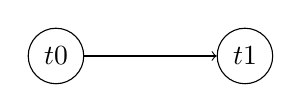
\begin{tikzpicture}[node distance = 3cm,scale=.8, every node/.style={circle,anchor=west}]
			\node[draw] (v1) at (0,0) {$t0$};
			\node[draw] (v2) at (3,0) {$t1$};
			\draw[->] (v1) edge (v2) ;	
		\end{tikzpicture}
	\end{figure} 	
	
	\subsection*{7.1.3}
	If we use locks without 2PL, we got the schedule $s''$:\\
	\begin{center}
	    \begin{tabular}{l|l}
	\hline
	$t_0$ & $t_1$ \\
	\hline
	$wl_0(A)$ & \\
	$r_0(A)$ & \\
	$w_0(A)$& \\	
	$wu_0(A)$& \\
	 & $wl_1(A)$ \\
	 & $r_1(A)$\\
	 & $wu_1(A)$\\
	& $wl_1(B)$ \\
	& $r_1(B)$\\
	& $wu_1(B)$\\
	& $c_1$\\
	$wl_0(B)$ & \\
	$r_0(B)$ & \\
	$w_0(B)$& \\ 
	$wu_0(B)$& \\
	$c_0$& \\
	\hline
	\end{tabular}		
	\end{center}
	
where $DT(s'')=r_0(A)w_0(A)r_1(A)r_1(B)c_1 r_0(B)w_0(B)c_0$, and its conflict graph is cyclic with $conflict(DT(s''))=\lbrace(w_0(A),r_1(A)), (r_1(B), w_0(B)) \rbrace$. So the lock leads to a not conflict serializable schedule.	
	
	\subsection*{7.1.4}
	

	\section*{Exercise 7.2(Recovery)}
	\subsection*{7.2.1}
		
	\subsection*{7.2.2}
	
	\subsection*{7.2.3}
		
		
		
	\section*{Exercise 7.3(B+-tree Locking)}
	\subsection*{7.2.1}
		
	\subsection*{7.2.2}
	
	\subsection*{7.2.3}
	
\end{document}


















